\chapter{Конструкторский раздел}
В данном разделе описываются требования к разрабатываемому методу.
Рассматриваются особенности разрабатываемого  метода, его архитектура и описываются ключевые шаги метода в виде схем алгоритмов.
\section*{Требования к разрабатываемому методу}
Метод распознавания спортивных действий человека на видео с использованием локального дескриптора должен:
\begin{itemize}
	\item[---] принимать на вход видео в форматах mp4;
	\item[---] разбивать видеоролик на кадры;
	\item[---] вычислять для каждого кадра дескриптор точек интереса;
	\item[---] проводить классификацию полученных дескрипторов.	
\end{itemize}



\section{Проектирование метода распознавания}
Формализуем постановку задачи в виде IDEF0-диаграмм нулевого и первого уровня и опишем входные и выходные данные метода распознавания спортивных действий человека на видео. Рассмотрим каждый из этапов реализации метода распознавания спортивных действий человека на видео. Для каждого этапа предоставляется схема алгоритма, решающая задачу, поставленную на этом этапе, а также более подробно описываются действия, представленные на схемах.
\subsection{IDEF0}

На рисунке 2.1 представлена диаграмма IDEF0 метода распознавания спортивных действий человека нулевого уровня.
\clearpage
\begin{figure}[h]
	\begin{center}
		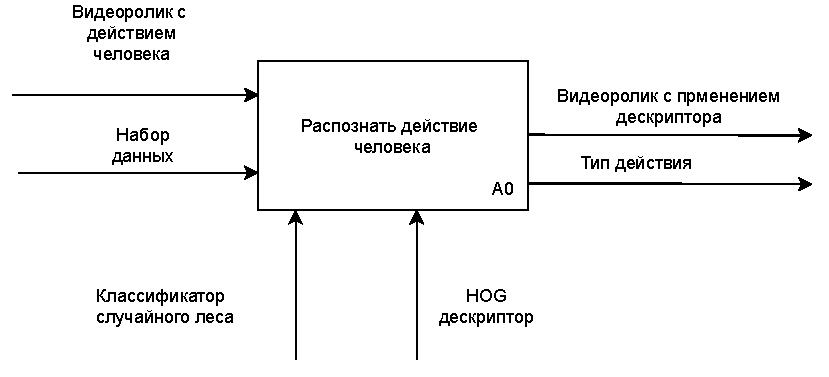
\includegraphics[ scale=1]{./img/idef0.pdf}
		\caption{IDEF0 нулевого уровня}  
		\label{fig:xray1}
	\end{center}
\end{figure}

На вход методу поступает набор данных для обучения модели и видео, которое после предобработки поступает на вход функции формирования дескриптора.
Также кадры видео, полученные в результате предобработки видео поступают на вход функции формирования исходного видео с наложенными градиентами интенсивностей. Полученные дескрипторы передаются на вход классификатора. На выходе метода: предсказанный тип действия и видео с градиентами интенсивностей.

На рисунке 2.2 представлена диаграмма IDEF0 разрабатываемого метода первого уровня.

\begin{figure}[h]
	\begin{center}
		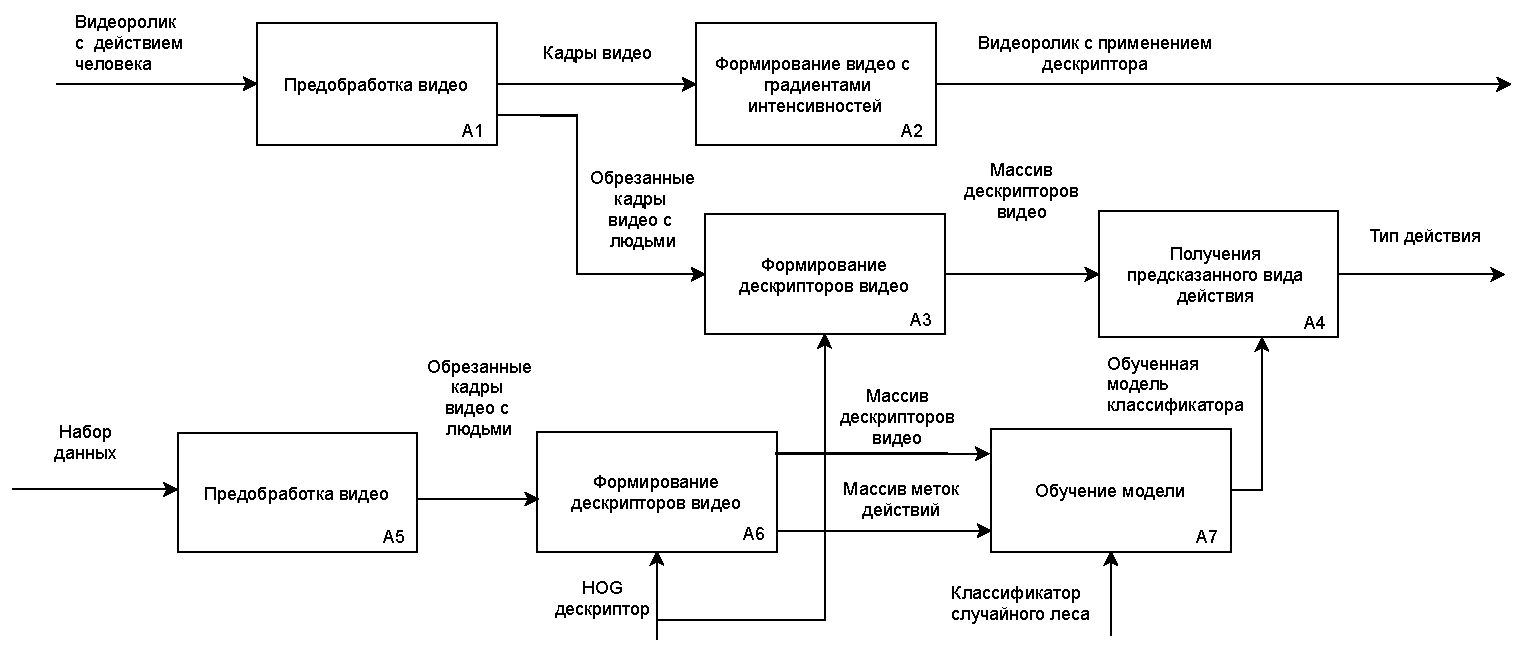
\includegraphics[ scale=0.68]{./img/idef1.pdf}
		\caption{IDEF0 первого уровня}  
		\label{fig:xray1}
	\end{center}
\end{figure}


\subsection{Предобработка видеоролика}

Для того, чтобы классифицировать действие человека на видео, необходимо разделить видеоролик на кадры для дальнейшей их обработки. \newline Для получения кадров необходимо определить частоту кадров (FPS -- frames per second). Частота кадров показывает сколько раз изображение появляется на экране в течение секунды. На рисунке 2.3 представлен алгоритм получение кадров видео.

\begin{figure}[h]
	\begin{center}
		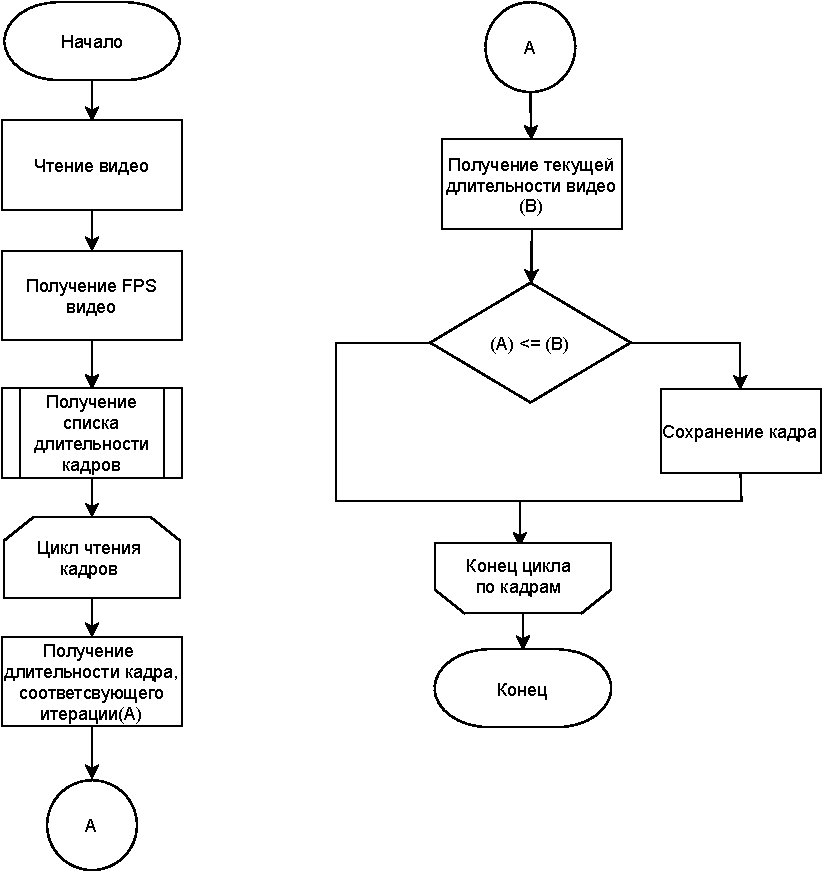
\includegraphics[ scale=1.1]{./img/frame.pdf}
		\caption{Алгоритм формирования кадров видео}  
		\label{fig:xray1}
	\end{center}
\end{figure}
\clearpage
Для более точного распознавания необходимо получать дескриптор не всего кадра, а его части, в котором находится человек. Это обусловлено тем, что без обрезания кадра дескриптор будет больше по размеру и иметь ненужные данные, которые негативно повлияют на результат обучения модели. Так же для того, чтобы обеспечить корректную работу алгоритма HOG в случае если размер кадра видео не кратен 16, необходимо изменить его размер на кратный 16, так как алгоритм вычисляет гистограмму ориентированных градиентов, разбивая изображения на области 16x16 пикселей. На рисунке 2.4 представлен алгоритм обрезания кадра. 
\begin{figure}[h]
	\begin{center}
		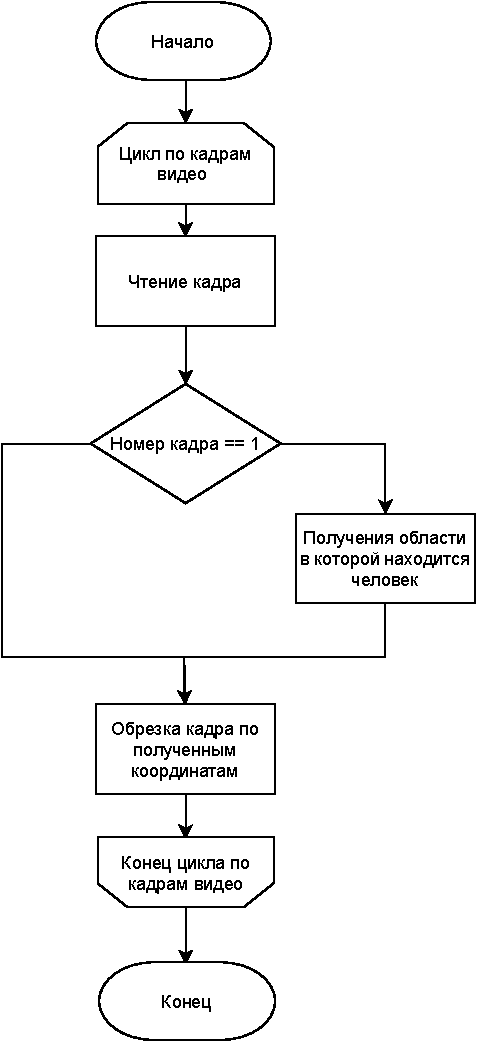
\includegraphics[ scale=0.9]{./img/man.pdf}
		\caption{Алгоритм обрезания кадра}  
		\label{fig:xray1}
	\end{center}
\end{figure}

\subsection{Формирование HOG дескриптора видео}
Для обучения модели, способной делать предсказания типа действия, совершаемого человеком на видео, необходимо сформировать дескрипторы видео, которые состоят из дескрипторов всех кадров данного видео. Дескриптор кадра представляет собой объединение гистограмм ориентированных градиентов, полученных для каждого блока кадра размером 16х16 пикселей. Гистограмма является вектором 36х1. Процесс формирования гистограмм подробно описан в разделе \ref{hog}.

%в главе 1.3.4 (HOG Гистограмма направленных градиентов).


%Чтобы нормализовать вектор, необходимо разделить каждое из этих значений на квадратный корень из суммы квадратов %значений. Вектор гистограммы ориентированных нрадиентов V:

%$V = [ a_{1} a_{2} a_{3} ... a_{36}]$

%Корень суммы квадратов:

%$k =\sqrt{}(a1)^2 + (a2)^2 + (a3)^2 + .... +(A36)^2$

%Для получения нормализованного вектора необходимо разделить все значения в векторе V на значение k.

В результате для каждого видео будет сформирован дескриптор, состоящий из гистограмм ориентированных градиентов, с помощью которых можно будет определить силуэт человека и  вид действия, который совершает человек.
На рисунке 2.5 представлен алгоритм формирование HOG дескриптора видео.
\clearpage
\begin{figure}[h]
	\begin{center}
		\centering
		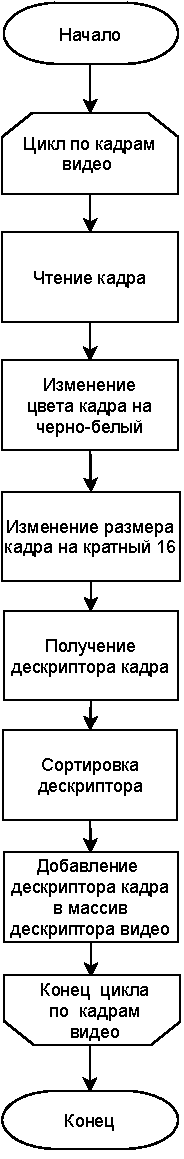
\includegraphics[ scale=1.1]{./img/descriptor.pdf}
		\caption{Алгоритм формирование HOG дескриптора}  
		\label{fig:xray1}
	\end{center}
\end{figure}
\clearpage
\subsection{Обучение модели}
Обучающая выборка видеороликов должна была пройти этап предобработки, после которого формировались данные для обучения, а именно дескрипторы видео и метки соответствующих действий.
Проинициализовав модель классификатора, ей передаются данные полученные в результате формирование дескрипторов. И после обучения файл готовой модели сохраняется. В качестве классификатора используется модель случайного леса.

Алгоритм построения случайного леса, состоящего из $\large N$ деревьев, выглядит следующим образом:


Для каждого $\large n = 1, \dots, N$:



\begin{itemize}
	\item[---] сгенерировать выборку $\large X_n$ с помощью бутстрэпа;
	\item[---] построить решающее дерево $\large b_n$ по выборке $\large X_n$:
		\begin{itemize}
			\item[---] по заданному критерию выбирается лучший признак, происходит разбиение дерева по этому критерию и так до исчерпания выборки;
			\item[---] дерево строится, пока в каждом листе не более $\large n_\text{min}$ объектов или пока не достигается определенная высота дерева;
			\item[---] при каждом разбиении сначала выбирается $\large m$ случайных признаков из $\large n$ исходных,
			и оптимальное разделение выборки ищется только среди них.
			
		\end{itemize}
	
\end{itemize}

Формула итогового классификатора:

\begin{equation}
\large a(x) = \frac{1}{N}\sum_{i = 1}^N b_i(x).
\end{equation}

Для задачи классификации результат определяется  голосованием по большинству.

Алгоритм получения обученной модели представлен на рисунке 2.6.
\clearpage

\begin{figure}[h]
	\begin{center}
		\centering
		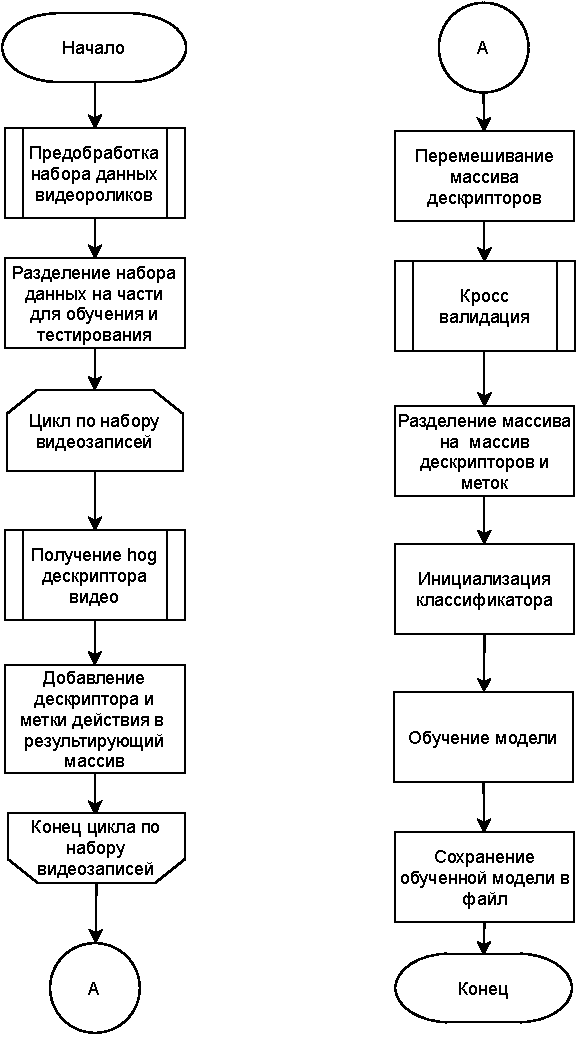
\includegraphics[ scale=1.1]{./img/module2.pdf}
		\caption{Алгоритм получения обученной модели}  
		\label{fig:xray1}
	\end{center}
\end{figure}
\clearpage
Алгоритм кросс-валидации (перекрестной проверки) предназначен для оценки качества работы модели. На рисунке 2.7 представлен этот алгоритм.

\begin{figure}[h]
	\begin{center}
		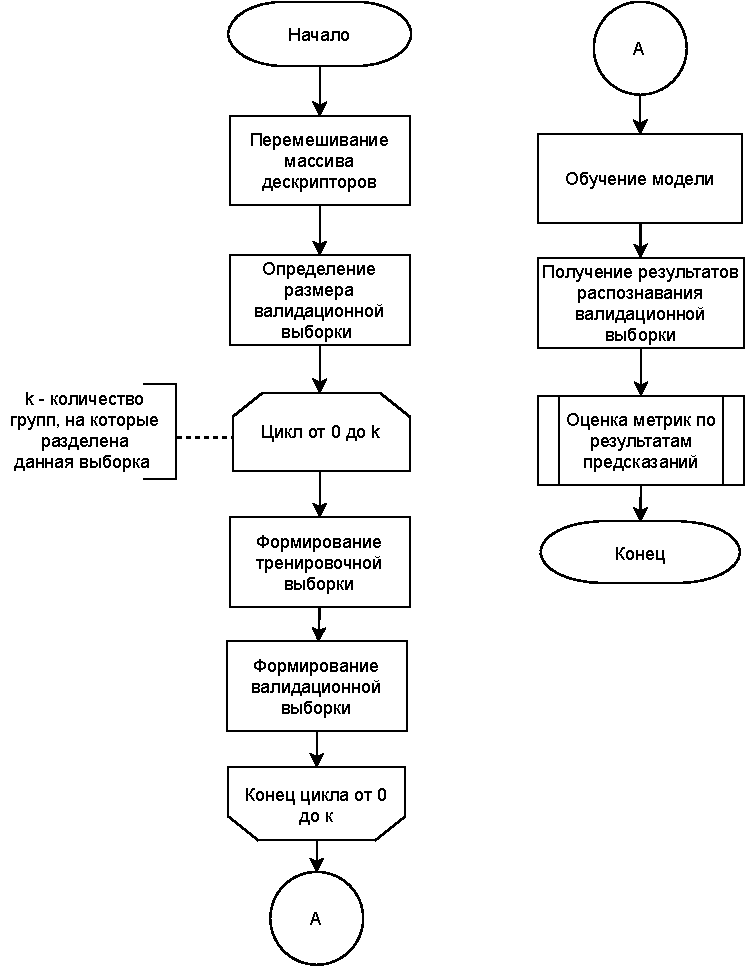
\includegraphics[ scale=1.1]{./img/val.pdf}
		\caption{Алгоритм k-fold кросс-валидации}  
		\label{fig:xray1}
	\end{center}
\end{figure}
\clearpage
\section{Набор данных}

Набор данных на котором будет обучаться модель был собран из трех открытых наборов данных:

\begin{itemize}
	\item[---] UCF101 -- это набор данных для распознавания действий, состоящий из реалистичных видеороликов, собранных с YouTube и имеющих 101 категорию действий. UCF101 обеспечивает наибольшее разнообразие с точки зрения действий и с наличием больших различий в движении камеры, внешнем виде объекта и позе, масштабе объекта, точке обзора, загроможденном фоне, условиях освещения и т.д.;
	\item[---] Набор данных HMDB51 представляет собой большую коллекцию реалистичных видеороликов из различных источников, включая фильмы и веб-видео. Набор данных состоит из 6766 видеоклипов из 51 категории действий, причем каждая категория содержит не менее 101 клипа;
	\item[---] Kinetics400 -- это набор данных для распознавания действий, состоящий из реалистичных видеороликов, собранных с YouTube. С 306 245 короткими обрезанными видеороликами из 400 категорий действий, это один из крупнейших и наиболее широко используемых наборов данных в исследовательском сообществе для сравнения современных моделей распознавания видео действий.
	
\end{itemize}

Так как наборы данных  содержат множество разных видов действий среди них, необходимо было выбрать различные фитнес упражнения. Итоговая выборка, на которой происходило обучение модели, содержит следующие виды спортивных действий:

\begin{itemize}
	\item[---] мостик (108 видео);
	\item[---] поднятие рук (330 видео);
	\item[---] джампинг джек (123 видео);
	\item[---] выпады (211 видео);
	\item[---] подтягивания (178 видео);
	\item[---] отжимания (139 видео);
	\item[---] пресс (146 видео);
	\item[---] приседания (122 видео);
	\item[---] растяжка ног (154 видео);	
	\item[---] махи ногами (129 видео).
\end{itemize}

Всего выборка содержит 1650 видео в списке выше указанно конкретное количество видео содержащий каждый класс действий. Перед обучением модели выборка была разделена в отношение 70\% для обучения и 30\% для тестирования.


\section*{Вывод}
Были представлены требования к разрабатываемому методу распознавания спортивных действий человека на видео.
Обозначены особенности разрабатываемого  метода, его архитектура и описаны ключевые шаги метода в виде схем алгоритмов.
Описана структура выбранного набора данных для обучения модели.
